\documentclass[1p]{elsarticle_modified}
%\bibliographystyle{elsarticle-num}

%\usepackage[colorlinks]{hyperref}
%\usepackage{abbrmath_seonhwa} %\Abb, \Ascr, \Acal ,\Abf, \Afrak
\usepackage{amsfonts}
\usepackage{amssymb}
\usepackage{amsmath}
\usepackage{amsthm}
\usepackage{scalefnt}
\usepackage{amsbsy}
\usepackage{kotex}
\usepackage{caption}
\usepackage{subfig}
\usepackage{color}
\usepackage{graphicx}
\usepackage{xcolor} %% white, black, red, green, blue, cyan, magenta, yellow
\usepackage{float}
\usepackage{setspace}
\usepackage{hyperref}

\usepackage{tikz}
\usetikzlibrary{arrows}

\usepackage{multirow}
\usepackage{array} % fixed length table
\usepackage{hhline}

%%%%%%%%%%%%%%%%%%%%%
\makeatletter
\renewcommand*\env@matrix[1][\arraystretch]{%
	\edef\arraystretch{#1}%
	\hskip -\arraycolsep
	\let\@ifnextchar\new@ifnextchar
	\array{*\c@MaxMatrixCols c}}
\makeatother %https://tex.stackexchange.com/questions/14071/how-can-i-increase-the-line-spacing-in-a-matrix
%%%%%%%%%%%%%%%

\usepackage[normalem]{ulem}

\newcommand{\msout}[1]{\ifmmode\text{\sout{\ensuremath{#1}}}\else\sout{#1}\fi}
%SOURCE: \msout is \stkout macro in https://tex.stackexchange.com/questions/20609/strikeout-in-math-mode

\newcommand{\cancel}[1]{
	\ifmmode
	{\color{red}\msout{#1}}
	\else
	{\color{red}\sout{#1}}
	\fi
}

\newcommand{\add}[1]{
	{\color{blue}\uwave{#1}}
}

\newcommand{\replace}[2]{
	\ifmmode
	{\color{red}\msout{#1}}{\color{blue}\uwave{#2}}
	\else
	{\color{red}\sout{#1}}{\color{blue}\uwave{#2}}
	\fi
}

\newcommand{\Sol}{\mathcal{S}} %segment
\newcommand{\D}{D} %diagram
\newcommand{\A}{\mathcal{A}} %arc


%%%%%%%%%%%%%%%%%%%%%%%%%%%%%5 test

\def\sl{\operatorname{\textup{SL}}(2,\Cbb)}
\def\psl{\operatorname{\textup{PSL}}(2,\Cbb)}
\def\quan{\mkern 1mu \triangleright \mkern 1mu}

\theoremstyle{definition}
\newtheorem{thm}{Theorem}[section]
\newtheorem{prop}[thm]{Proposition}
\newtheorem{lem}[thm]{Lemma}
\newtheorem{ques}[thm]{Question}
\newtheorem{cor}[thm]{Corollary}
\newtheorem{defn}[thm]{Definition}
\newtheorem{exam}[thm]{Example}
\newtheorem{rmk}[thm]{Remark}
\newtheorem{alg}[thm]{Algorithm}

\newcommand{\I}{\sqrt{-1}}
\begin{document}

%\begin{frontmatter}
%
%\title{Boundary parabolic representations of knots up to 8 crossings}
%
%%% Group authors per affiliation:
%\author{Yunhi Cho} 
%\address{Department of Mathematics, University of Seoul, Seoul, Korea}
%\ead{yhcho@uos.ac.kr}
%
%
%\author{Seonhwa Kim} %\fnref{s_kim}}
%\address{Center for Geometry and Physics, Institute for Basic Science, Pohang, 37673, Korea}
%\ead{ryeona17@ibs.re.kr}
%
%\author{Hyuk Kim}
%\address{Department of Mathematical Sciences, Seoul National University, Seoul 08826, Korea}
%\ead{hyukkim@snu.ac.kr}
%
%\author{Seokbeom Yoon}
%\address{Department of Mathematical Sciences, Seoul National University, Seoul, 08826,  Korea}
%\ead{sbyoon15@snu.ac.kr}
%
%\begin{abstract}
%We find all boundary parabolic representation of knots up to 8 crossings.
%
%\end{abstract}
%\begin{keyword}
%    \MSC[2010] 57M25 
%\end{keyword}
%
%\end{frontmatter}

%\linenumbers
%\tableofcontents
%
\newcommand\colored[1]{\textcolor{white}{\rule[-0.35ex]{0.8em}{1.4ex}}\kern-0.8em\color{red} #1}%
%\newcommand\colored[1]{\textcolor{white}{ #1}\kern-2.17ex	\textcolor{white}{ #1}\kern-1.81ex	\textcolor{white}{ #1}\kern-2.15ex\color{red}#1	}

{\Large $\underline{12n_{0794}~(K12n_{0794})}$}

\setlength{\tabcolsep}{10pt}
\renewcommand{\arraystretch}{1.6}
\vspace{1cm}\begin{tabular}{m{100pt}>{\centering\arraybackslash}m{274pt}}
\multirow{5}{120pt}{
	\centering
	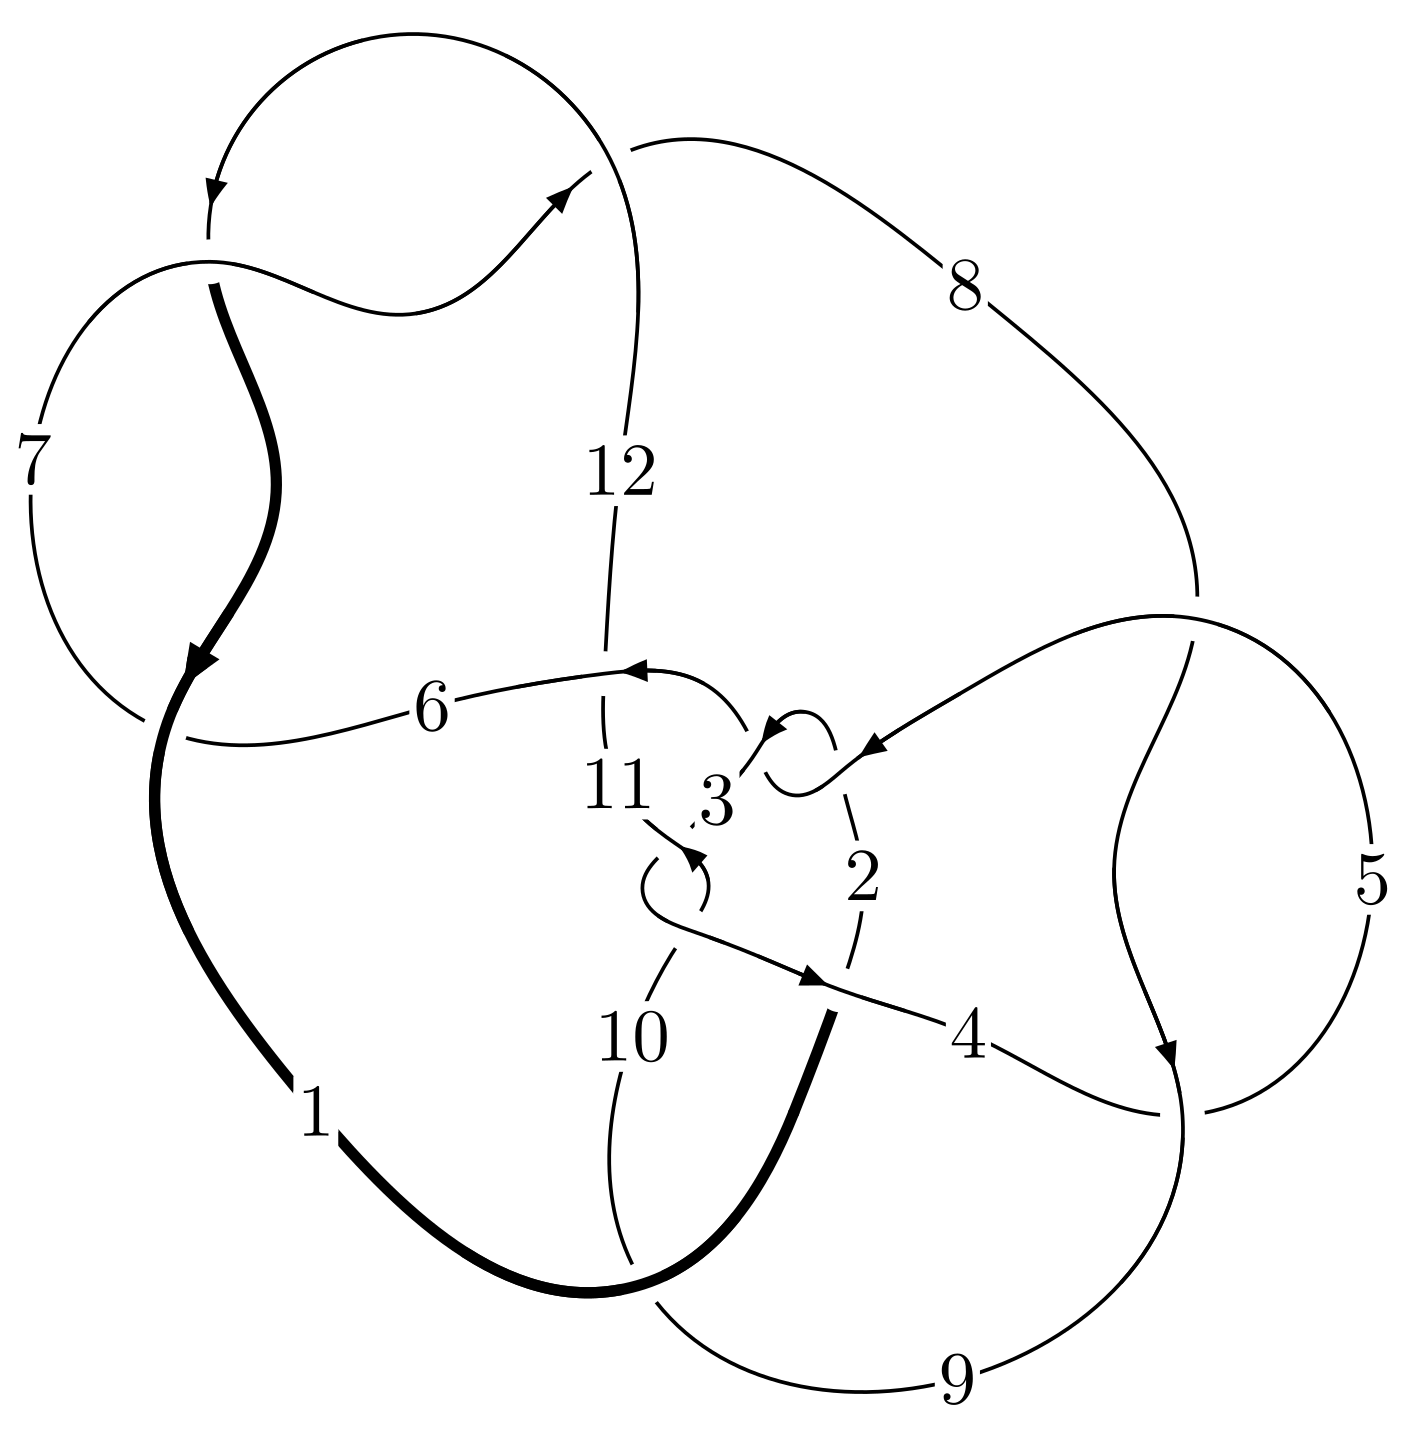
\includegraphics[width=112pt]{../../../GIT/diagram.site/Diagrams/png/2883_12n_0794.png}\\
\ \ \ A knot diagram\footnotemark}&
\allowdisplaybreaks
\textbf{Linearized knot diagam} \\
\cline{2-2}
 &
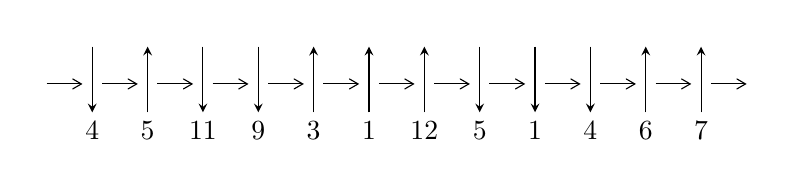
\begin{tikzpicture}[x=20pt, y=17pt]
	% nodes
	\node (C0) at (0, 0) {};
	\node (C1) at (1, 0) {};
	\node (C1U) at (1, +1) {};
	\node (C1D) at (1, -1) {4};

	\node (C2) at (2, 0) {};
	\node (C2U) at (2, +1) {};
	\node (C2D) at (2, -1) {5};

	\node (C3) at (3, 0) {};
	\node (C3U) at (3, +1) {};
	\node (C3D) at (3, -1) {11};

	\node (C4) at (4, 0) {};
	\node (C4U) at (4, +1) {};
	\node (C4D) at (4, -1) {9};

	\node (C5) at (5, 0) {};
	\node (C5U) at (5, +1) {};
	\node (C5D) at (5, -1) {3};

	\node (C6) at (6, 0) {};
	\node (C6U) at (6, +1) {};
	\node (C6D) at (6, -1) {1};

	\node (C7) at (7, 0) {};
	\node (C7U) at (7, +1) {};
	\node (C7D) at (7, -1) {12};

	\node (C8) at (8, 0) {};
	\node (C8U) at (8, +1) {};
	\node (C8D) at (8, -1) {5};

	\node (C9) at (9, 0) {};
	\node (C9U) at (9, +1) {};
	\node (C9D) at (9, -1) {1};

	\node (C10) at (10, 0) {};
	\node (C10U) at (10, +1) {};
	\node (C10D) at (10, -1) {4};

	\node (C11) at (11, 0) {};
	\node (C11U) at (11, +1) {};
	\node (C11D) at (11, -1) {6};

	\node (C12) at (12, 0) {};
	\node (C12U) at (12, +1) {};
	\node (C12D) at (12, -1) {7};
	\node (C13) at (13, 0) {};

	% arrows
	\draw[->,>={angle 60}]
	(C0) edge (C1) (C1) edge (C2) (C2) edge (C3) (C3) edge (C4) (C4) edge (C5) (C5) edge (C6) (C6) edge (C7) (C7) edge (C8) (C8) edge (C9) (C9) edge (C10) (C10) edge (C11) (C11) edge (C12) (C12) edge (C13) ;	\draw[->,>=stealth]
	(C1U) edge (C1D) (C2D) edge (C2U) (C3U) edge (C3D) (C4U) edge (C4D) (C5D) edge (C5U) (C6D) edge (C6U) (C7D) edge (C7U) (C8U) edge (C8D) (C9U) edge (C9D) (C10U) edge (C10D) (C11D) edge (C11U) (C12D) edge (C12U) ;
	\end{tikzpicture} \\
\hhline{~~} \\& 
\textbf{Solving Sequence} \\ \cline{2-2} 
 &
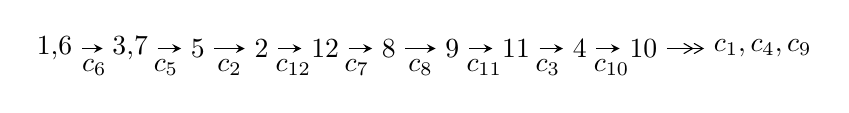
\begin{tikzpicture}[x=23pt, y=7pt]
	% node
	\node (A0) at (-1/8, 0) {1,6};
	\node (A1) at (17/16, 0) {3,7};
	\node (A2) at (17/8, 0) {5};
	\node (A3) at (25/8, 0) {2};
	\node (A4) at (33/8, 0) {12};
	\node (A5) at (41/8, 0) {8};
	\node (A6) at (49/8, 0) {9};
	\node (A7) at (57/8, 0) {11};
	\node (A8) at (65/8, 0) {4};
	\node (A9) at (73/8, 0) {10};
	\node (C1) at (1/2, -1) {$c_{6}$};
	\node (C2) at (13/8, -1) {$c_{5}$};
	\node (C3) at (21/8, -1) {$c_{2}$};
	\node (C4) at (29/8, -1) {$c_{12}$};
	\node (C5) at (37/8, -1) {$c_{7}$};
	\node (C6) at (45/8, -1) {$c_{8}$};
	\node (C7) at (53/8, -1) {$c_{11}$};
	\node (C8) at (61/8, -1) {$c_{3}$};
	\node (C9) at (69/8, -1) {$c_{10}$};
	\node (A10) at (11, 0) {$c_{1},c_{4},c_{9}$};

	% edge
	\draw[->,>=stealth]	
	(A0) edge (A1) (A1) edge (A2) (A2) edge (A3) (A3) edge (A4) (A4) edge (A5) (A5) edge (A6) (A6) edge (A7) (A7) edge (A8) (A8) edge (A9) ;
	\draw[->>,>={angle 60}]	
	(A9) edge (A10);
\end{tikzpicture} \\ 

\end{tabular} \\

\footnotetext{
The image of knot diagram is generated by the software ``\textbf{Draw programme}" developed by Andrew Bartholomew(\url{http://www.layer8.co.uk/maths/draw/index.htm\#Running-draw}), where we modified some parts for our purpose(\url{https://github.com/CATsTAILs/LinksPainter}).
}\phantom \\ \newline 
\centering \textbf{Ideals for irreducible components\footnotemark of $X_{\text{par}}$} 
 
\begin{align*}
I^u_{1}&=\langle 
3.64825\times10^{60} u^{67}+2.17531\times10^{61} u^{66}+\cdots+2.27197\times10^{61} b+3.17348\times10^{62},\\
\phantom{I^u_{1}}&\phantom{= \langle  }-3.41778\times10^{61} u^{67}+4.19437\times10^{61} u^{66}+\cdots+4.31675\times10^{62} a-8.54844\times10^{62},\\
\phantom{I^u_{1}}&\phantom{= \langle  }u^{68}+32 u^{66}+\cdots-17 u+19\rangle \\
I^u_{2}&=\langle 
u^{17}+u^{16}+\cdots+b+3 u,\;u^{16}- u^{15}+\cdots+a-1,\;u^{18}+u^{17}+\cdots+2 u+1\rangle \\
\\
\end{align*}
\raggedright * 2 irreducible components of $\dim_{\mathbb{C}}=0$, with total 86 representations.\\
\footnotetext{All coefficients of polynomials are rational numbers. But the coefficients are sometimes approximated in decimal forms when there is not enough margin.}
\newpage
\renewcommand{\arraystretch}{1}
\centering \section*{I. $I^u_{1}= \langle 3.65\times10^{60} u^{67}+2.18\times10^{61} u^{66}+\cdots+2.27\times10^{61} b+3.17\times10^{62},\;-3.42\times10^{61} u^{67}+4.19\times10^{61} u^{66}+\cdots+4.32\times10^{62} a-8.55\times10^{62},\;u^{68}+32 u^{66}+\cdots-17 u+19 \rangle$}
\flushleft \textbf{(i) Arc colorings}\\
\begin{tabular}{m{7pt} m{180pt} m{7pt} m{180pt} }
\flushright $a_{1}=$&$\begin{pmatrix}0\\u\end{pmatrix}$ \\
\flushright $a_{6}=$&$\begin{pmatrix}1\\0\end{pmatrix}$ \\
\flushright $a_{3}=$&$\begin{pmatrix}0.0791748 u^{67}-0.0971649 u^{66}+\cdots+7.13718 u+1.98030\\-0.160576 u^{67}-0.957454 u^{66}+\cdots+5.17375 u-13.9679\end{pmatrix}$ \\
\flushright $a_{7}=$&$\begin{pmatrix}1\\- u^2\end{pmatrix}$ \\
\flushright $a_{5}=$&$\begin{pmatrix}0.434570 u^{67}+0.198997 u^{66}+\cdots-3.14705 u-2.64483\\-0.802804 u^{67}-0.137974 u^{66}+\cdots-6.93147 u-0.143677\end{pmatrix}$ \\
\flushright $a_{2}=$&$\begin{pmatrix}-0.221569 u^{67}-0.256066 u^{66}+\cdots-4.45414 u-5.67050\\-0.431397 u^{67}-0.300463 u^{66}+\cdots+0.0481534 u-2.05464\end{pmatrix}$ \\
\flushright $a_{12}=$&$\begin{pmatrix}- u\\u^3+u\end{pmatrix}$ \\
\flushright $a_{8}=$&$\begin{pmatrix}u^2+1\\- u^4-2 u^2\end{pmatrix}$ \\
\flushright $a_{9}=$&$\begin{pmatrix}0.0300223 u^{67}-0.192535 u^{66}+\cdots+1.41247 u-0.794270\\-0.541452 u^{67}+1.19433 u^{66}+\cdots-21.1227 u+14.5984\end{pmatrix}$ \\
\flushright $a_{11}=$&$\begin{pmatrix}- u^3-2 u\\u^3+u\end{pmatrix}$ \\
\flushright $a_{4}=$&$\begin{pmatrix}-0.254863 u^{67}-0.559737 u^{66}+\cdots+5.39514 u-4.47736\\-0.0427600 u^{67}-1.30834 u^{66}+\cdots+10.9051 u-18.4670\end{pmatrix}$ \\
\flushright $a_{10}=$&$\begin{pmatrix}0.0300223 u^{67}-0.192535 u^{66}+\cdots+1.41247 u-0.794270\\-0.757625 u^{67}+1.35968 u^{66}+\cdots-24.9663 u+18.2566\end{pmatrix}$\\&\end{tabular}
\flushleft \textbf{(ii) Obstruction class $= -1$}\\~\\
\flushleft \textbf{(iii) Cusp Shapes $= -0.759415 u^{67}-2.10567 u^{66}+\cdots+23.3339 u-15.4588$}\\~\\
\newpage\renewcommand{\arraystretch}{1}
\flushleft \textbf{(iv) u-Polynomials at the component}\newline \\
\begin{tabular}{m{50pt}|m{274pt}}
Crossings & \hspace{64pt}u-Polynomials at each crossing \\
\hline $$\begin{aligned}c_{1}\end{aligned}$$&$\begin{aligned}
&u^{68}-6 u^{67}+\cdots-27 u+1
\end{aligned}$\\
\hline $$\begin{aligned}c_{2},c_{5}\end{aligned}$$&$\begin{aligned}
&u^{68}-2 u^{67}+\cdots-2106 u+1161
\end{aligned}$\\
\hline $$\begin{aligned}c_{3},c_{10}\end{aligned}$$&$\begin{aligned}
&u^{68}- u^{67}+\cdots+430 u+55
\end{aligned}$\\
\hline $$\begin{aligned}c_{4},c_{8}\end{aligned}$$&$\begin{aligned}
&u^{68}+2 u^{67}+\cdots+157 u+31
\end{aligned}$\\
\hline $$\begin{aligned}c_{6},c_{7},c_{12}\end{aligned}$$&$\begin{aligned}
&u^{68}+32 u^{66}+\cdots+17 u+19
\end{aligned}$\\
\hline $$\begin{aligned}c_{9}\end{aligned}$$&$\begin{aligned}
&u^{68}+4 u^{67}+\cdots- u+1
\end{aligned}$\\
\hline $$\begin{aligned}c_{11}\end{aligned}$$&$\begin{aligned}
&u^{68}-2 u^{65}+\cdots-109361 u+34447
\end{aligned}$\\
\hline
\end{tabular}\\~\\
\newpage\renewcommand{\arraystretch}{1}
\flushleft \textbf{(v) Riley Polynomials at the component}\newline \\
\begin{tabular}{m{50pt}|m{274pt}}
Crossings & \hspace{64pt}Riley Polynomials at each crossing \\
\hline $$\begin{aligned}c_{1}\end{aligned}$$&$\begin{aligned}
&y^{68}-54 y^{67}+\cdots+189 y+1
\end{aligned}$\\
\hline $$\begin{aligned}c_{2},c_{5}\end{aligned}$$&$\begin{aligned}
&y^{68}-34 y^{67}+\cdots-27367308 y+1347921
\end{aligned}$\\
\hline $$\begin{aligned}c_{3},c_{10}\end{aligned}$$&$\begin{aligned}
&y^{68}+25 y^{67}+\cdots+220450 y+3025
\end{aligned}$\\
\hline $$\begin{aligned}c_{4},c_{8}\end{aligned}$$&$\begin{aligned}
&y^{68}+24 y^{67}+\cdots+22223 y+961
\end{aligned}$\\
\hline $$\begin{aligned}c_{6},c_{7},c_{12}\end{aligned}$$&$\begin{aligned}
&y^{68}+64 y^{67}+\cdots-2075 y+361
\end{aligned}$\\
\hline $$\begin{aligned}c_{9}\end{aligned}$$&$\begin{aligned}
&y^{68}-50 y^{67}+\cdots+217 y+1
\end{aligned}$\\
\hline $$\begin{aligned}c_{11}\end{aligned}$$&$\begin{aligned}
&y^{68}+46 y^{66}+\cdots+15032565303 y+1186595809
\end{aligned}$\\
\hline
\end{tabular}\\~\\
\newpage\flushleft \textbf{(vi) Complex Volumes and Cusp Shapes}
$$\begin{array}{c|c|c}  
\text{Solutions to }I^u_{1}& \I (\text{vol} + \sqrt{-1}CS) & \text{Cusp shape}\\
 \hline 
\begin{aligned}
u &= \phantom{-}0.585021 + 0.839577 I \\
a &= -0.653745 + 0.824312 I \\
b &= \phantom{-}1.156370 - 0.575904 I\end{aligned}
 & -0.92653 - 6.48550 I & \phantom{-0.000000 } 0 \\ \hline\begin{aligned}
u &= \phantom{-}0.585021 - 0.839577 I \\
a &= -0.653745 - 0.824312 I \\
b &= \phantom{-}1.156370 + 0.575904 I\end{aligned}
 & -0.92653 + 6.48550 I & \phantom{-0.000000 } 0 \\ \hline\begin{aligned}
u &= \phantom{-}0.844238 + 0.314098 I \\
a &= -2.05637 + 0.11980 I \\
b &= \phantom{-}1.29281 + 0.70336 I\end{aligned}
 & \phantom{-}0.71987 + 11.42660 I & \phantom{-}2.99478 - 7.86086 I \\ \hline\begin{aligned}
u &= \phantom{-}0.844238 - 0.314098 I \\
a &= -2.05637 - 0.11980 I \\
b &= \phantom{-}1.29281 - 0.70336 I\end{aligned}
 & \phantom{-}0.71987 - 11.42660 I & \phantom{-}2.99478 + 7.86086 I \\ \hline\begin{aligned}
u &= -0.774174 + 0.442382 I \\
a &= -1.73133 - 0.65078 I \\
b &= \phantom{-}1.280470 - 0.119995 I\end{aligned}
 & \phantom{-}4.56836 - 2.47145 I & \phantom{-}9.7968 + 11.8051 I \\ \hline\begin{aligned}
u &= -0.774174 - 0.442382 I \\
a &= -1.73133 + 0.65078 I \\
b &= \phantom{-}1.280470 + 0.119995 I\end{aligned}
 & \phantom{-}4.56836 + 2.47145 I & \phantom{-}9.7968 - 11.8051 I \\ \hline\begin{aligned}
u &= -0.601969 + 0.651291 I \\
a &= \phantom{-}0.198331 + 0.799993 I \\
b &= -0.865200 - 0.503209 I\end{aligned}
 & -1.65284 - 0.01935 I & \phantom{-}0.571143 + 0.160005 I \\ \hline\begin{aligned}
u &= -0.601969 - 0.651291 I \\
a &= \phantom{-}0.198331 - 0.799993 I \\
b &= -0.865200 + 0.503209 I\end{aligned}
 & -1.65284 + 0.01935 I & \phantom{-}0.571143 - 0.160005 I \\ \hline\begin{aligned}
u &= -0.878561 + 0.090514 I \\
a &= -1.54583 - 0.41382 I \\
b &= \phantom{-}0.864053 - 0.090063 I\end{aligned}
 & \phantom{-}3.96123 - 0.33995 I & \phantom{-}6.36296 - 1.08101 I \\ \hline\begin{aligned}
u &= -0.878561 - 0.090514 I \\
a &= -1.54583 + 0.41382 I \\
b &= \phantom{-}0.864053 + 0.090063 I\end{aligned}
 & \phantom{-}3.96123 + 0.33995 I & \phantom{-}6.36296 + 1.08101 I\\
 \hline 
 \end{array}$$\newpage$$\begin{array}{c|c|c}  
\text{Solutions to }I^u_{1}& \I (\text{vol} + \sqrt{-1}CS) & \text{Cusp shape}\\
 \hline 
\begin{aligned}
u &= -0.761968 + 0.375228 I \\
a &= \phantom{-}1.51651 + 0.13278 I \\
b &= -1.057950 + 0.707192 I\end{aligned}
 & -0.72761 - 4.58564 I & \phantom{-}1.01495 + 4.58399 I \\ \hline\begin{aligned}
u &= -0.761968 - 0.375228 I \\
a &= \phantom{-}1.51651 - 0.13278 I \\
b &= -1.057950 - 0.707192 I\end{aligned}
 & -0.72761 + 4.58564 I & \phantom{-}1.01495 - 4.58399 I \\ \hline\begin{aligned}
u &= \phantom{-}0.087906 + 1.195280 I \\
a &= -1.036050 - 0.725247 I \\
b &= \phantom{-}1.336380 - 0.253283 I\end{aligned}
 & \phantom{-}4.71460 + 0.88214 I & \phantom{-0.000000 } 0 \\ \hline\begin{aligned}
u &= \phantom{-}0.087906 - 1.195280 I \\
a &= -1.036050 + 0.725247 I \\
b &= \phantom{-}1.336380 + 0.253283 I\end{aligned}
 & \phantom{-}4.71460 - 0.88214 I & \phantom{-0.000000 } 0 \\ \hline\begin{aligned}
u &= \phantom{-}0.046584 + 1.212660 I \\
a &= -0.563907 + 1.049470 I \\
b &= -0.263145 + 1.187020 I\end{aligned}
 & -4.47402 - 2.56568 I & \phantom{-0.000000 } 0 \\ \hline\begin{aligned}
u &= \phantom{-}0.046584 - 1.212660 I \\
a &= -0.563907 - 1.049470 I \\
b &= -0.263145 - 1.187020 I\end{aligned}
 & -4.47402 + 2.56568 I & \phantom{-0.000000 } 0 \\ \hline\begin{aligned}
u &= \phantom{-}0.776255 + 0.084754 I \\
a &= \phantom{-}1.96737 + 0.45778 I \\
b &= -1.044090 - 0.751566 I\end{aligned}
 & \phantom{-}4.20666 + 3.23614 I & \phantom{-}6.34201 - 8.24044 I \\ \hline\begin{aligned}
u &= \phantom{-}0.776255 - 0.084754 I \\
a &= \phantom{-}1.96737 - 0.45778 I \\
b &= -1.044090 + 0.751566 I\end{aligned}
 & \phantom{-}4.20666 - 3.23614 I & \phantom{-}6.34201 + 8.24044 I \\ \hline\begin{aligned}
u &= -0.109251 + 1.214890 I \\
a &= \phantom{-}0.80584 + 2.16972 I \\
b &= -0.484418 - 0.064884 I\end{aligned}
 & -4.41125 + 1.64954 I & \phantom{-0.000000 } 0 \\ \hline\begin{aligned}
u &= -0.109251 - 1.214890 I \\
a &= \phantom{-}0.80584 - 2.16972 I \\
b &= -0.484418 + 0.064884 I\end{aligned}
 & -4.41125 - 1.64954 I & \phantom{-0.000000 } 0\\
 \hline 
 \end{array}$$\newpage$$\begin{array}{c|c|c}  
\text{Solutions to }I^u_{1}& \I (\text{vol} + \sqrt{-1}CS) & \text{Cusp shape}\\
 \hline 
\begin{aligned}
u &= \phantom{-}0.320207 + 1.177390 I \\
a &= \phantom{-}0.418143 - 0.634187 I \\
b &= -1.087520 + 0.478535 I\end{aligned}
 & \phantom{-}0.881245 + 0.747708 I & \phantom{-0.000000 } 0 \\ \hline\begin{aligned}
u &= \phantom{-}0.320207 - 1.177390 I \\
a &= \phantom{-}0.418143 + 0.634187 I \\
b &= -1.087520 - 0.478535 I\end{aligned}
 & \phantom{-}0.881245 - 0.747708 I & \phantom{-0.000000 } 0 \\ \hline\begin{aligned}
u &= -0.489550 + 1.132460 I \\
a &= -0.845195 - 0.209506 I \\
b &= \phantom{-}0.961776 - 0.091917 I\end{aligned}
 & \phantom{-}0.75256 - 4.50250 I & \phantom{-0.000000 } 0 \\ \hline\begin{aligned}
u &= -0.489550 - 1.132460 I \\
a &= -0.845195 + 0.209506 I \\
b &= \phantom{-}0.961776 + 0.091917 I\end{aligned}
 & \phantom{-}0.75256 + 4.50250 I & \phantom{-0.000000 } 0 \\ \hline\begin{aligned}
u &= \phantom{-}0.168395 + 1.254750 I \\
a &= \phantom{-}0.909624 - 0.738354 I \\
b &= -1.68054 + 0.07433 I\end{aligned}
 & \phantom{-}1.09519 + 2.03459 I & \phantom{-0.000000 } 0 \\ \hline\begin{aligned}
u &= \phantom{-}0.168395 - 1.254750 I \\
a &= \phantom{-}0.909624 + 0.738354 I \\
b &= -1.68054 - 0.07433 I\end{aligned}
 & \phantom{-}1.09519 - 2.03459 I & \phantom{-0.000000 } 0 \\ \hline\begin{aligned}
u &= \phantom{-}0.622042 + 0.266962 I \\
a &= -0.333728 + 1.061650 I \\
b &= \phantom{-}0.328416 - 1.217050 I\end{aligned}
 & -2.34650 + 4.70127 I & \phantom{-}1.66541 - 6.89019 I \\ \hline\begin{aligned}
u &= \phantom{-}0.622042 - 0.266962 I \\
a &= -0.333728 - 1.061650 I \\
b &= \phantom{-}0.328416 + 1.217050 I\end{aligned}
 & -2.34650 - 4.70127 I & \phantom{-}1.66541 + 6.89019 I \\ \hline\begin{aligned}
u &= \phantom{-}0.201780 + 1.344270 I \\
a &= \phantom{-}0.47779 - 1.40922 I \\
b &= -1.357800 - 0.380695 I\end{aligned}
 & \phantom{-}0.11696 + 3.16123 I & \phantom{-0.000000 } 0 \\ \hline\begin{aligned}
u &= \phantom{-}0.201780 - 1.344270 I \\
a &= \phantom{-}0.47779 + 1.40922 I \\
b &= -1.357800 + 0.380695 I\end{aligned}
 & \phantom{-}0.11696 - 3.16123 I & \phantom{-0.000000 } 0\\
 \hline 
 \end{array}$$\newpage$$\begin{array}{c|c|c}  
\text{Solutions to }I^u_{1}& \I (\text{vol} + \sqrt{-1}CS) & \text{Cusp shape}\\
 \hline 
\begin{aligned}
u &= \phantom{-}0.331726 + 1.319540 I \\
a &= \phantom{-}1.35514 - 0.94546 I \\
b &= -1.019720 - 0.935363 I\end{aligned}
 & -0.19484 + 7.23478 I & \phantom{-0.000000 } 0 \\ \hline\begin{aligned}
u &= \phantom{-}0.331726 - 1.319540 I \\
a &= \phantom{-}1.35514 + 0.94546 I \\
b &= -1.019720 + 0.935363 I\end{aligned}
 & -0.19484 - 7.23478 I & \phantom{-0.000000 } 0 \\ \hline\begin{aligned}
u &= -0.380858 + 1.315350 I \\
a &= -0.930411 - 0.962245 I \\
b &= \phantom{-}0.739624 - 0.217715 I\end{aligned}
 & -0.42239 - 4.83795 I & \phantom{-0.000000 } 0 \\ \hline\begin{aligned}
u &= -0.380858 - 1.315350 I \\
a &= -0.930411 + 0.962245 I \\
b &= \phantom{-}0.739624 + 0.217715 I\end{aligned}
 & -0.42239 + 4.83795 I & \phantom{-0.000000 } 0 \\ \hline\begin{aligned}
u &= -0.580317 + 0.214057 I \\
a &= \phantom{-}3.38471 - 0.40273 I \\
b &= -0.891148 + 0.455999 I\end{aligned}
 & -1.63250 - 3.94273 I & \phantom{-}3.88858 + 5.95678 I \\ \hline\begin{aligned}
u &= -0.580317 - 0.214057 I \\
a &= \phantom{-}3.38471 + 0.40273 I \\
b &= -0.891148 - 0.455999 I\end{aligned}
 & -1.63250 + 3.94273 I & \phantom{-}3.88858 - 5.95678 I \\ \hline\begin{aligned}
u &= -0.084571 + 1.382930 I \\
a &= -0.054497 + 0.537587 I \\
b &= \phantom{-}0.045186 + 0.944137 I\end{aligned}
 & -5.41837 - 1.91442 I & \phantom{-0.000000 } 0 \\ \hline\begin{aligned}
u &= -0.084571 - 1.382930 I \\
a &= -0.054497 - 0.537587 I \\
b &= \phantom{-}0.045186 - 0.944137 I\end{aligned}
 & -5.41837 + 1.91442 I & \phantom{-0.000000 } 0 \\ \hline\begin{aligned}
u &= \phantom{-}0.562673 + 0.242422 I \\
a &= -0.55392 + 1.40968 I \\
b &= \phantom{-}0.920370 + 0.284651 I\end{aligned}
 & \phantom{-}7.32966 + 1.28471 I & \phantom{-}0.07472 - 6.09575 I \\ \hline\begin{aligned}
u &= \phantom{-}0.562673 - 0.242422 I \\
a &= -0.55392 - 1.40968 I \\
b &= \phantom{-}0.920370 - 0.284651 I\end{aligned}
 & \phantom{-}7.32966 - 1.28471 I & \phantom{-}0.07472 + 6.09575 I\\
 \hline 
 \end{array}$$\newpage$$\begin{array}{c|c|c}  
\text{Solutions to }I^u_{1}& \I (\text{vol} + \sqrt{-1}CS) & \text{Cusp shape}\\
 \hline 
\begin{aligned}
u &= -0.235874 + 1.386730 I \\
a &= \phantom{-}1.69465 + 0.80471 I \\
b &= -1.178050 + 0.518685 I\end{aligned}
 & -6.75272 - 6.96733 I & \phantom{-0.000000 } 0 \\ \hline\begin{aligned}
u &= -0.235874 - 1.386730 I \\
a &= \phantom{-}1.69465 - 0.80471 I \\
b &= -1.178050 - 0.518685 I\end{aligned}
 & -6.75272 + 6.96733 I & \phantom{-0.000000 } 0 \\ \hline\begin{aligned}
u &= -0.190501 + 1.394310 I \\
a &= -0.048935 - 0.246393 I \\
b &= -0.90235 - 1.14942 I\end{aligned}
 & -7.39171 - 0.99406 I & \phantom{-0.000000 } 0 \\ \hline\begin{aligned}
u &= -0.190501 - 1.394310 I \\
a &= -0.048935 + 0.246393 I \\
b &= -0.90235 + 1.14942 I\end{aligned}
 & -7.39171 + 0.99406 I & \phantom{-0.000000 } 0 \\ \hline\begin{aligned}
u &= \phantom{-}0.420221 + 0.405604 I \\
a &= -2.51276 - 0.10334 I \\
b &= \phantom{-}0.464174 + 0.701970 I\end{aligned}
 & -3.13089 - 1.54804 I & -1.36292 - 1.90908 I \\ \hline\begin{aligned}
u &= \phantom{-}0.420221 - 0.405604 I \\
a &= -2.51276 + 0.10334 I \\
b &= \phantom{-}0.464174 - 0.701970 I\end{aligned}
 & -3.13089 + 1.54804 I & -1.36292 + 1.90908 I \\ \hline\begin{aligned}
u &= \phantom{-}0.23300 + 1.40172 I \\
a &= \phantom{-}0.136138 + 1.020950 I \\
b &= \phantom{-}0.642226 + 0.477177 I\end{aligned}
 & \phantom{-}2.04560 + 4.25350 I & \phantom{-0.000000 } 0 \\ \hline\begin{aligned}
u &= \phantom{-}0.23300 - 1.40172 I \\
a &= \phantom{-}0.136138 - 1.020950 I \\
b &= \phantom{-}0.642226 - 0.477177 I\end{aligned}
 & \phantom{-}2.04560 - 4.25350 I & \phantom{-0.000000 } 0 \\ \hline\begin{aligned}
u &= \phantom{-}0.25005 + 1.40302 I \\
a &= \phantom{-}0.452465 - 0.063748 I \\
b &= \phantom{-}0.51101 - 1.40622 I\end{aligned}
 & -7.67530 + 7.91631 I & \phantom{-0.000000 } 0 \\ \hline\begin{aligned}
u &= \phantom{-}0.25005 - 1.40302 I \\
a &= \phantom{-}0.452465 + 0.063748 I \\
b &= \phantom{-}0.51101 + 1.40622 I\end{aligned}
 & -7.67530 - 7.91631 I & \phantom{-0.000000 } 0\\
 \hline 
 \end{array}$$\newpage$$\begin{array}{c|c|c}  
\text{Solutions to }I^u_{1}& \I (\text{vol} + \sqrt{-1}CS) & \text{Cusp shape}\\
 \hline 
\begin{aligned}
u &= \phantom{-}0.16140 + 1.41858 I \\
a &= -1.24247 + 0.74107 I \\
b &= \phantom{-}0.915024 + 0.747286 I\end{aligned}
 & -8.91641 + 0.61969 I & \phantom{-0.000000 } 0 \\ \hline\begin{aligned}
u &= \phantom{-}0.16140 - 1.41858 I \\
a &= -1.24247 - 0.74107 I \\
b &= \phantom{-}0.915024 - 0.747286 I\end{aligned}
 & -8.91641 - 0.61969 I & \phantom{-0.000000 } 0 \\ \hline\begin{aligned}
u &= \phantom{-}0.537783 + 0.087841 I \\
a &= \phantom{-}2.96586 - 1.04036 I \\
b &= -1.52148 - 0.18593 I\end{aligned}
 & \phantom{-}4.68996 + 0.46786 I & \phantom{-}7.22305 + 1.64442 I \\ \hline\begin{aligned}
u &= \phantom{-}0.537783 - 0.087841 I \\
a &= \phantom{-}2.96586 + 1.04036 I \\
b &= -1.52148 + 0.18593 I\end{aligned}
 & \phantom{-}4.68996 - 0.46786 I & \phantom{-}7.22305 - 1.64442 I \\ \hline\begin{aligned}
u &= -0.462909 + 0.260608 I \\
a &= \phantom{-}1.080330 + 0.319178 I \\
b &= -0.662469 - 0.970115 I\end{aligned}
 & -2.09947 + 1.48120 I & \phantom{-}2.08400 + 2.14333 I \\ \hline\begin{aligned}
u &= -0.462909 - 0.260608 I \\
a &= \phantom{-}1.080330 - 0.319178 I \\
b &= -0.662469 + 0.970115 I\end{aligned}
 & -2.09947 - 1.48120 I & \phantom{-}2.08400 - 2.14333 I \\ \hline\begin{aligned}
u &= \phantom{-}0.33871 + 1.44643 I \\
a &= -1.15336 + 1.08090 I \\
b &= \phantom{-}1.34420 + 0.82627 I\end{aligned}
 & -4.9007 + 15.7068 I & \phantom{-0.000000 } 0 \\ \hline\begin{aligned}
u &= \phantom{-}0.33871 - 1.44643 I \\
a &= -1.15336 - 1.08090 I \\
b &= \phantom{-}1.34420 - 0.82627 I\end{aligned}
 & -4.9007 - 15.7068 I & \phantom{-0.000000 } 0 \\ \hline\begin{aligned}
u &= -0.30870 + 1.45326 I \\
a &= -0.867601 - 0.899252 I \\
b &= \phantom{-}1.274760 - 0.368438 I\end{aligned}
 & -1.42486 - 6.45156 I & \phantom{-0.000000 } 0 \\ \hline\begin{aligned}
u &= -0.30870 - 1.45326 I \\
a &= -0.867601 + 0.899252 I \\
b &= \phantom{-}1.274760 + 0.368438 I\end{aligned}
 & -1.42486 + 6.45156 I & \phantom{-0.000000 } 0\\
 \hline 
 \end{array}$$\newpage$$\begin{array}{c|c|c}  
\text{Solutions to }I^u_{1}& \I (\text{vol} + \sqrt{-1}CS) & \text{Cusp shape}\\
 \hline 
\begin{aligned}
u &= -0.29407 + 1.45891 I \\
a &= \phantom{-}0.812866 + 0.905342 I \\
b &= -1.08796 + 0.91104 I\end{aligned}
 & -6.61106 - 8.42932 I & \phantom{-0.000000 } 0 \\ \hline\begin{aligned}
u &= -0.29407 - 1.45891 I \\
a &= \phantom{-}0.812866 - 0.905342 I \\
b &= -1.08796 - 0.91104 I\end{aligned}
 & -6.61106 + 8.42932 I & \phantom{-0.000000 } 0 \\ \hline\begin{aligned}
u &= -0.15940 + 1.55376 I \\
a &= -0.323360 + 0.186562 I \\
b &= -0.528474 - 0.501666 I\end{aligned}
 & -8.96596 - 2.72922 I & \phantom{-0.000000 } 0 \\ \hline\begin{aligned}
u &= -0.15940 - 1.55376 I \\
a &= -0.323360 - 0.186562 I \\
b &= -0.528474 + 0.501666 I\end{aligned}
 & -8.96596 + 2.72922 I & \phantom{-0.000000 } 0 \\ \hline\begin{aligned}
u &= -0.226546 + 0.361814 I \\
a &= -0.207356 + 0.203335 I \\
b &= -0.236794 + 0.345165 I\end{aligned}
 & \phantom{-}0.028670 - 0.891534 I & \phantom{-}0.60339 + 7.68948 I \\ \hline\begin{aligned}
u &= -0.226546 - 0.361814 I \\
a &= -0.207356 - 0.203335 I \\
b &= -0.236794 - 0.345165 I\end{aligned}
 & \phantom{-}0.028670 + 0.891534 I & \phantom{-}0.60339 - 7.68948 I \\ \hline\begin{aligned}
u &= \phantom{-}0.05123 + 1.58208 I \\
a &= \phantom{-}0.0639758 + 0.0036631 I \\
b &= \phantom{-}0.792248 - 0.599111 I\end{aligned}
 & -9.31745 - 4.59027 I & \phantom{-0.000000 } 0 \\ \hline\begin{aligned}
u &= \phantom{-}0.05123 - 1.58208 I \\
a &= \phantom{-}0.0639758 - 0.0036631 I \\
b &= \phantom{-}0.792248 + 0.599111 I\end{aligned}
 & -9.31745 + 4.59027 I & \phantom{-0.000000 } 0\\
 \hline 
 \end{array}$$\newpage\newpage\renewcommand{\arraystretch}{1}
\centering \section*{II. $I^u_{2}= \langle u^{17}+u^{16}+\cdots+b+3 u,\;u^{16}- u^{15}+\cdots+a-1,\;u^{18}+u^{17}+\cdots+2 u+1 \rangle$}
\flushleft \textbf{(i) Arc colorings}\\
\begin{tabular}{m{7pt} m{180pt} m{7pt} m{180pt} }
\flushright $a_{1}=$&$\begin{pmatrix}0\\u\end{pmatrix}$ \\
\flushright $a_{6}=$&$\begin{pmatrix}1\\0\end{pmatrix}$ \\
\flushright $a_{3}=$&$\begin{pmatrix}- u^{16}+u^{15}+\cdots+9 u+1\\- u^{17}- u^{16}+\cdots-2 u^2-3 u\end{pmatrix}$ \\
\flushright $a_{7}=$&$\begin{pmatrix}1\\- u^2\end{pmatrix}$ \\
\flushright $a_{5}=$&$\begin{pmatrix}- u^{17}- u^{16}+\cdots-8 u^2+3\\- u^{17}+u^{16}+\cdots+u+1\end{pmatrix}$ \\
\flushright $a_{2}=$&$\begin{pmatrix}2 u^{17}+18 u^{15}+\cdots-12 u^2+15 u\\- u^{17}-3 u^{16}+\cdots-5 u-1\end{pmatrix}$ \\
\flushright $a_{12}=$&$\begin{pmatrix}- u\\u^3+u\end{pmatrix}$ \\
\flushright $a_{8}=$&$\begin{pmatrix}u^2+1\\- u^4-2 u^2\end{pmatrix}$ \\
\flushright $a_{9}=$&$\begin{pmatrix}-2 u^{17}-2 u^{16}+\cdots-12 u-2\\u^{17}+u^{16}+\cdots-2 u^2+2 u\end{pmatrix}$ \\
\flushright $a_{11}=$&$\begin{pmatrix}- u^3-2 u\\u^3+u\end{pmatrix}$ \\
\flushright $a_{4}=$&$\begin{pmatrix}- u^{16}+u^{15}+\cdots+10 u+1\\- u^{15}- u^{14}+\cdots- u^3-3 u\end{pmatrix}$ \\
\flushright $a_{10}=$&$\begin{pmatrix}-2 u^{17}-2 u^{16}+\cdots-12 u-2\\2 u^{17}+2 u^{16}+\cdots+7 u^3+4 u\end{pmatrix}$\\&\end{tabular}
\flushleft \textbf{(ii) Obstruction class $= 1$}\\~\\
\flushleft \textbf{(iii) Cusp Shapes $= - u^{17}+10 u^{16}+2 u^{15}+84 u^{14}+52 u^{13}+276 u^{12}+194 u^{11}+420 u^{10}+292 u^9+227 u^8+135 u^7-85 u^6-84 u^5-67 u^4-54 u^3+53 u^2+25 u+11$}\\~\\
\newpage\renewcommand{\arraystretch}{1}
\flushleft \textbf{(iv) u-Polynomials at the component}\newline \\
\begin{tabular}{m{50pt}|m{274pt}}
Crossings & \hspace{64pt}u-Polynomials at each crossing \\
\hline $$\begin{aligned}c_{1}\end{aligned}$$&$\begin{aligned}
&u^{18}-3 u^{17}+\cdots+4 u^2+1
\end{aligned}$\\
\hline $$\begin{aligned}c_{2}\end{aligned}$$&$\begin{aligned}
&u^{18}+3 u^{17}+\cdots+3 u+1
\end{aligned}$\\
\hline $$\begin{aligned}c_{3}\end{aligned}$$&$\begin{aligned}
&u^{18}+6 u^{16}+\cdots- u+1
\end{aligned}$\\
\hline $$\begin{aligned}c_{4}\end{aligned}$$&$\begin{aligned}
&u^{18}+u^{17}+\cdots+9 u^2+1
\end{aligned}$\\
\hline $$\begin{aligned}c_{5}\end{aligned}$$&$\begin{aligned}
&u^{18}-3 u^{17}+\cdots-3 u+1
\end{aligned}$\\
\hline $$\begin{aligned}c_{6},c_{7}\end{aligned}$$&$\begin{aligned}
&u^{18}+u^{17}+\cdots+2 u+1
\end{aligned}$\\
\hline $$\begin{aligned}c_{8}\end{aligned}$$&$\begin{aligned}
&u^{18}- u^{17}+\cdots+9 u^2+1
\end{aligned}$\\
\hline $$\begin{aligned}c_{9}\end{aligned}$$&$\begin{aligned}
&u^{18}+u^{17}+\cdots+6 u^2+1
\end{aligned}$\\
\hline $$\begin{aligned}c_{10}\end{aligned}$$&$\begin{aligned}
&u^{18}+6 u^{16}+\cdots+u+1
\end{aligned}$\\
\hline $$\begin{aligned}c_{11}\end{aligned}$$&$\begin{aligned}
&u^{18}+u^{17}+\cdots+7 u^2+1
\end{aligned}$\\
\hline $$\begin{aligned}c_{12}\end{aligned}$$&$\begin{aligned}
&u^{18}- u^{17}+\cdots-2 u+1
\end{aligned}$\\
\hline
\end{tabular}\\~\\
\newpage\renewcommand{\arraystretch}{1}
\flushleft \textbf{(v) Riley Polynomials at the component}\newline \\
\begin{tabular}{m{50pt}|m{274pt}}
Crossings & \hspace{64pt}Riley Polynomials at each crossing \\
\hline $$\begin{aligned}c_{1}\end{aligned}$$&$\begin{aligned}
&y^{18}-11 y^{17}+\cdots+8 y+1
\end{aligned}$\\
\hline $$\begin{aligned}c_{2},c_{5}\end{aligned}$$&$\begin{aligned}
&y^{18}-15 y^{17}+\cdots+3 y+1
\end{aligned}$\\
\hline $$\begin{aligned}c_{3},c_{10}\end{aligned}$$&$\begin{aligned}
&y^{18}+12 y^{17}+\cdots-3 y+1
\end{aligned}$\\
\hline $$\begin{aligned}c_{4},c_{8}\end{aligned}$$&$\begin{aligned}
&y^{18}+15 y^{17}+\cdots+18 y+1
\end{aligned}$\\
\hline $$\begin{aligned}c_{6},c_{7},c_{12}\end{aligned}$$&$\begin{aligned}
&y^{18}+19 y^{17}+\cdots+12 y+1
\end{aligned}$\\
\hline $$\begin{aligned}c_{9}\end{aligned}$$&$\begin{aligned}
&y^{18}-3 y^{17}+\cdots+12 y+1
\end{aligned}$\\
\hline $$\begin{aligned}c_{11}\end{aligned}$$&$\begin{aligned}
&y^{18}- y^{17}+\cdots+14 y+1
\end{aligned}$\\
\hline
\end{tabular}\\~\\
\newpage\flushleft \textbf{(vi) Complex Volumes and Cusp Shapes}
$$\begin{array}{c|c|c}  
\text{Solutions to }I^u_{2}& \I (\text{vol} + \sqrt{-1}CS) & \text{Cusp shape}\\
 \hline 
\begin{aligned}
u &= -0.773934 + 0.231488 I \\
a &= -2.08394 - 0.31153 I \\
b &= \phantom{-}1.282150 - 0.263447 I\end{aligned}
 & \phantom{-}4.46749 - 1.83303 I & \phantom{-}7.57936 + 0.69386 I \\ \hline\begin{aligned}
u &= -0.773934 - 0.231488 I \\
a &= -2.08394 + 0.31153 I \\
b &= \phantom{-}1.282150 + 0.263447 I\end{aligned}
 & \phantom{-}4.46749 + 1.83303 I & \phantom{-}7.57936 - 0.69386 I \\ \hline\begin{aligned}
u &= -0.214946 + 1.181900 I \\
a &= -0.677293 - 1.058070 I \\
b &= \phantom{-}1.59277 + 0.19212 I\end{aligned}
 & \phantom{-}1.81304 - 1.52738 I & \phantom{-}7.36454 + 0.16276 I \\ \hline\begin{aligned}
u &= -0.214946 - 1.181900 I \\
a &= -0.677293 + 1.058070 I \\
b &= \phantom{-}1.59277 - 0.19212 I\end{aligned}
 & \phantom{-}1.81304 + 1.52738 I & \phantom{-}7.36454 - 0.16276 I \\ \hline\begin{aligned}
u &= \phantom{-}0.207784 + 1.231320 I \\
a &= \phantom{-}1.113550 + 0.166807 I \\
b &= -1.303010 + 0.187111 I\end{aligned}
 & \phantom{-}4.69100 + 1.96995 I & \phantom{-}2.62542 - 4.79081 I \\ \hline\begin{aligned}
u &= \phantom{-}0.207784 - 1.231320 I \\
a &= \phantom{-}1.113550 - 0.166807 I \\
b &= -1.303010 - 0.187111 I\end{aligned}
 & \phantom{-}4.69100 - 1.96995 I & \phantom{-}2.62542 + 4.79081 I \\ \hline\begin{aligned}
u &= -0.038102 + 1.259780 I \\
a &= \phantom{-}0.48564 + 1.79761 I \\
b &= \phantom{-}0.318175 + 0.845570 I\end{aligned}
 & -5.44116 + 2.12330 I & -7.44188 - 2.77053 I \\ \hline\begin{aligned}
u &= -0.038102 - 1.259780 I \\
a &= \phantom{-}0.48564 - 1.79761 I \\
b &= \phantom{-}0.318175 - 0.845570 I\end{aligned}
 & -5.44116 - 2.12330 I & -7.44188 + 2.77053 I \\ \hline\begin{aligned}
u &= \phantom{-}0.622411 + 0.160441 I \\
a &= \phantom{-}1.46043 - 1.42137 I \\
b &= -1.086800 - 0.210154 I\end{aligned}
 & \phantom{-}7.94870 + 0.94161 I & \phantom{-}11.28164 - 0.01284 I \\ \hline\begin{aligned}
u &= \phantom{-}0.622411 - 0.160441 I \\
a &= \phantom{-}1.46043 + 1.42137 I \\
b &= -1.086800 + 0.210154 I\end{aligned}
 & \phantom{-}7.94870 - 0.94161 I & \phantom{-}11.28164 + 0.01284 I\\
 \hline 
 \end{array}$$\newpage$$\begin{array}{c|c|c}  
\text{Solutions to }I^u_{2}& \I (\text{vol} + \sqrt{-1}CS) & \text{Cusp shape}\\
 \hline 
\begin{aligned}
u &= -0.370236 + 1.364330 I \\
a &= -1.119980 - 0.827045 I \\
b &= \phantom{-}1.088670 - 0.482755 I\end{aligned}
 & -0.53522 - 6.08319 I & \phantom{-}2.90511 + 6.25752 I \\ \hline\begin{aligned}
u &= -0.370236 - 1.364330 I \\
a &= -1.119980 + 0.827045 I \\
b &= \phantom{-}1.088670 + 0.482755 I\end{aligned}
 & -0.53522 + 6.08319 I & \phantom{-}2.90511 - 6.25752 I \\ \hline\begin{aligned}
u &= \phantom{-}0.27236 + 1.38898 I \\
a &= \phantom{-}0.169437 - 1.185730 I \\
b &= -0.899855 - 0.319836 I\end{aligned}
 & \phantom{-}2.95502 + 4.25254 I & \phantom{-}5.77944 - 3.56884 I \\ \hline\begin{aligned}
u &= \phantom{-}0.27236 - 1.38898 I \\
a &= \phantom{-}0.169437 + 1.185730 I \\
b &= -0.899855 + 0.319836 I\end{aligned}
 & \phantom{-}2.95502 - 4.25254 I & \phantom{-}5.77944 + 3.56884 I \\ \hline\begin{aligned}
u &= -0.07316 + 1.53250 I \\
a &= \phantom{-}0.048434 + 0.355139 I \\
b &= \phantom{-}0.205474 - 0.413665 I\end{aligned}
 & -8.72912 - 3.55791 I & -0.20761 + 3.94043 I \\ \hline\begin{aligned}
u &= -0.07316 - 1.53250 I \\
a &= \phantom{-}0.048434 - 0.355139 I \\
b &= \phantom{-}0.205474 + 0.413665 I\end{aligned}
 & -8.72912 + 3.55791 I & -0.20761 - 3.94043 I \\ \hline\begin{aligned}
u &= -0.132177 + 0.304356 I \\
a &= \phantom{-}0.60372 + 3.51396 I \\
b &= \phantom{-}0.302437 - 0.618636 I\end{aligned}
 & -2.23494 - 2.68244 I & \phantom{-}2.11398 + 3.46850 I \\ \hline\begin{aligned}
u &= -0.132177 - 0.304356 I \\
a &= \phantom{-}0.60372 - 3.51396 I \\
b &= \phantom{-}0.302437 + 0.618636 I\end{aligned}
 & -2.23494 + 2.68244 I & \phantom{-}2.11398 - 3.46850 I\\
 \hline 
 \end{array}$$\newpage
\newpage\renewcommand{\arraystretch}{1}
\centering \section*{ III. u-Polynomials}
\begin{tabular}{m{50pt}|m{274pt}}
Crossings & \hspace{64pt}u-Polynomials at each crossing \\
\hline $$\begin{aligned}c_{1}\end{aligned}$$&$\begin{aligned}
&(u^{18}-3 u^{17}+\cdots+4 u^2+1)(u^{68}-6 u^{67}+\cdots-27 u+1)
\end{aligned}$\\
\hline $$\begin{aligned}c_{2}\end{aligned}$$&$\begin{aligned}
&(u^{18}+3 u^{17}+\cdots+3 u+1)(u^{68}-2 u^{67}+\cdots-2106 u+1161)
\end{aligned}$\\
\hline $$\begin{aligned}c_{3}\end{aligned}$$&$\begin{aligned}
&(u^{18}+6 u^{16}+\cdots- u+1)(u^{68}- u^{67}+\cdots+430 u+55)
\end{aligned}$\\
\hline $$\begin{aligned}c_{4}\end{aligned}$$&$\begin{aligned}
&(u^{18}+u^{17}+\cdots+9 u^2+1)(u^{68}+2 u^{67}+\cdots+157 u+31)
\end{aligned}$\\
\hline $$\begin{aligned}c_{5}\end{aligned}$$&$\begin{aligned}
&(u^{18}-3 u^{17}+\cdots-3 u+1)(u^{68}-2 u^{67}+\cdots-2106 u+1161)
\end{aligned}$\\
\hline $$\begin{aligned}c_{6},c_{7}\end{aligned}$$&$\begin{aligned}
&(u^{18}+u^{17}+\cdots+2 u+1)(u^{68}+32 u^{66}+\cdots+17 u+19)
\end{aligned}$\\
\hline $$\begin{aligned}c_{8}\end{aligned}$$&$\begin{aligned}
&(u^{18}- u^{17}+\cdots+9 u^2+1)(u^{68}+2 u^{67}+\cdots+157 u+31)
\end{aligned}$\\
\hline $$\begin{aligned}c_{9}\end{aligned}$$&$\begin{aligned}
&(u^{18}+u^{17}+\cdots+6 u^2+1)(u^{68}+4 u^{67}+\cdots- u+1)
\end{aligned}$\\
\hline $$\begin{aligned}c_{10}\end{aligned}$$&$\begin{aligned}
&(u^{18}+6 u^{16}+\cdots+u+1)(u^{68}- u^{67}+\cdots+430 u+55)
\end{aligned}$\\
\hline $$\begin{aligned}c_{11}\end{aligned}$$&$\begin{aligned}
&(u^{18}+u^{17}+\cdots+7 u^2+1)(u^{68}-2 u^{65}+\cdots-109361 u+34447)
\end{aligned}$\\
\hline $$\begin{aligned}c_{12}\end{aligned}$$&$\begin{aligned}
&(u^{18}- u^{17}+\cdots-2 u+1)(u^{68}+32 u^{66}+\cdots+17 u+19)
\end{aligned}$\\
\hline
\end{tabular}\newpage\renewcommand{\arraystretch}{1}
\centering \section*{ IV. Riley Polynomials}
\begin{tabular}{m{50pt}|m{274pt}}
Crossings & \hspace{64pt}Riley Polynomials at each crossing \\
\hline $$\begin{aligned}c_{1}\end{aligned}$$&$\begin{aligned}
&(y^{18}-11 y^{17}+\cdots+8 y+1)(y^{68}-54 y^{67}+\cdots+189 y+1)
\end{aligned}$\\
\hline $$\begin{aligned}c_{2},c_{5}\end{aligned}$$&$\begin{aligned}
&(y^{18}-15 y^{17}+\cdots+3 y+1)\\
&\cdot(y^{68}-34 y^{67}+\cdots-27367308 y+1347921)
\end{aligned}$\\
\hline $$\begin{aligned}c_{3},c_{10}\end{aligned}$$&$\begin{aligned}
&(y^{18}+12 y^{17}+\cdots-3 y+1)(y^{68}+25 y^{67}+\cdots+220450 y+3025)
\end{aligned}$\\
\hline $$\begin{aligned}c_{4},c_{8}\end{aligned}$$&$\begin{aligned}
&(y^{18}+15 y^{17}+\cdots+18 y+1)(y^{68}+24 y^{67}+\cdots+22223 y+961)
\end{aligned}$\\
\hline $$\begin{aligned}c_{6},c_{7},c_{12}\end{aligned}$$&$\begin{aligned}
&(y^{18}+19 y^{17}+\cdots+12 y+1)(y^{68}+64 y^{67}+\cdots-2075 y+361)
\end{aligned}$\\
\hline $$\begin{aligned}c_{9}\end{aligned}$$&$\begin{aligned}
&(y^{18}-3 y^{17}+\cdots+12 y+1)(y^{68}-50 y^{67}+\cdots+217 y+1)
\end{aligned}$\\
\hline $$\begin{aligned}c_{11}\end{aligned}$$&$\begin{aligned}
&(y^{18}- y^{17}+\cdots+14 y+1)\\
&\cdot(y^{68}+46 y^{66}+\cdots+15032565303 y+1186595809)
\end{aligned}$\\
\hline
\end{tabular}
\vskip 2pc
\end{document}